\section{User Research}\label{sect:UserResearch}

\subsection{Introduction}\label{subsect:UR_Introduction}
Following the market and competitor analysis, the next fundamental step in the design process of TrainHub was conducting comprehensive User Research. As established by the theoretical principles of mobile interaction design, engaging directly with potential users is crucial to fully understand their real needs, daily habits, and primary frustrations. 

To gather both quantitative and qualitative data, we designed and distributed a targeted questionnaire using Google Forms. Recognizing the dual-sided nature of our platform, the survey was carefully structured to accommodate differentiated paths for our two main user categories: gym members (clients) and fitness professionals (admins). 

The primary objective of this research phase was twofold: first, to empirically validate our initial assumptions regarding the preliminary features; second, to uncover the actual pain points caused by the current digital fragmentation in the fitness industry. The insights gathered from this questionnaire provided the necessary data-driven foundation to define realistic User Personas and formulate concrete User Scenarios, ultimately guiding the design and development of the application's interface.

\subsection{Questionnaire and Results}\label{subsect:QuestionnaireResults}
To empirically validate our design hypothesis, the Google Forms survey was distributed to a varied sample of individuals involved in the fitness ecosystem. The questionnaire collected a total of 76 valid responses. By utilizing conditional logic branches within the form, we ensured that both gym members and professionals could provide specific, highly relevant insights based on their distinct operational contexts.

\subsubsection{Demographics}\label{subsubsect:Demographics}

\begin{figure}[H]
    \centering
    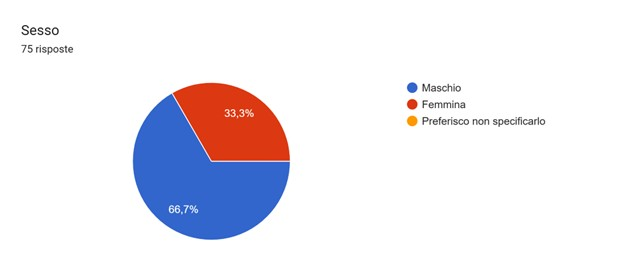
\includegraphics[width=0.8\textwidth]{3-UserResearch/img/Questionnaire/Demographics/Sesso.jpg}
    \caption{Gender distribution of the respondents.}
    \label{img:QuestionnaireGender}
\end{figure}

\begin{figure}[H]
    \centering
    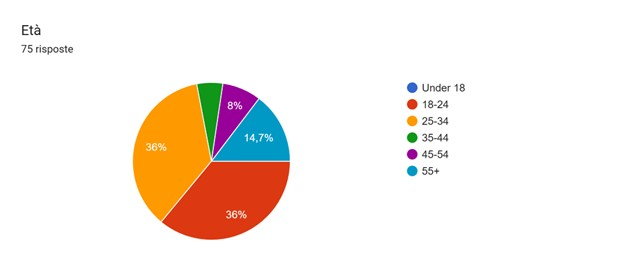
\includegraphics[width=0.8\textwidth]{3-UserResearch/img/Questionnaire/Demographics/Eta.jpg}
    \caption{Age distribution of the respondents.}
    \label{img:QuestionnaireAge}
\end{figure}

\begin{figure}[H]
    \centering
    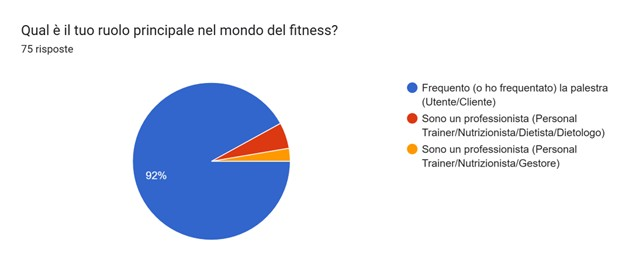
\includegraphics[width=0.8\textwidth]{3-UserResearch/img/Questionnaire/Demographics/Ruolo.jpg}
    \caption{Role distribution of the respondents.}
    \label{img:QuestionnaireRole}
\end{figure}

\textbf{Note: }The red and orange categories in the legend of Figure \ref{img:QuestionnaireRole} were split by Google Forms, but they actually represent the same group.

\vspace{0.3cm}
\textbf{Analysis of Demographics:} 
As shown in Figures \ref{img:QuestionnaireGender} and \ref{img:QuestionnaireAge}, the demographic profile of the respondents indicates a predominantly young adult audience, with the vast majority falling into the 18-24 and 25-34 age brackets. The sample of 76 respondents successfully captured insights from both sides of the market: exactly 92\% (70 individuals) identified as gym members (clients), while the remaining 8\% (6 individuals) are certified professionals (Personal Trainers, Nutritionists, and Dietitians). This specific distribution strongly mirrors the realistic proportions of a physical gym ecosystem, where a smaller, dedicated group of staff members manages a high volume of clients, ensuring that our feedback accurately reflects real-world market dynamics.


\subsubsection{Gym Members' Feedback}\label{subsubsect:GymMembers'Feedback}

\begin{figure}[H]
    \centering
    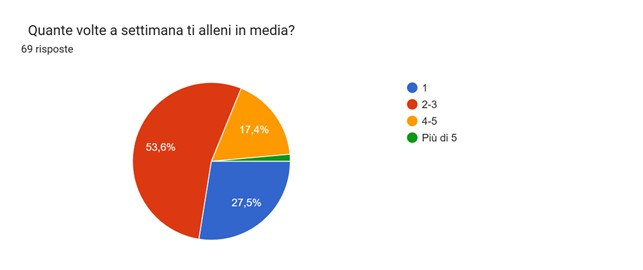
\includegraphics[width=0.8\textwidth]{3-UserResearch/img/Questionnaire/GymMembers/FrequenzaAllenamento.jpg}
    \caption{Frequency of training sessions.}
    \label{img:QuestionnaireFrequency}
\end{figure}

\begin{figure}[H]
    \centering
    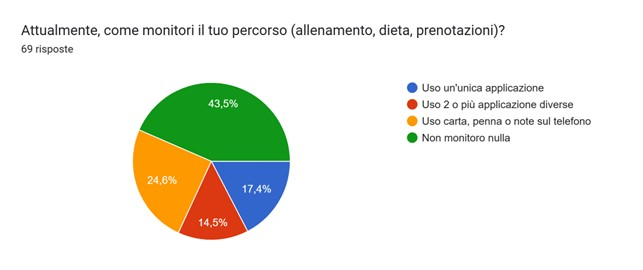
\includegraphics[width=0.8\textwidth]{3-UserResearch/img/Questionnaire/GymMembers/MonitoraggioAllenamento.jpg}
    \caption{Methods used by gym members to track their training sessions.}
    \label{img:QuestionnaireTracking}
\end{figure}

\begin{figure}[H]
    \centering
    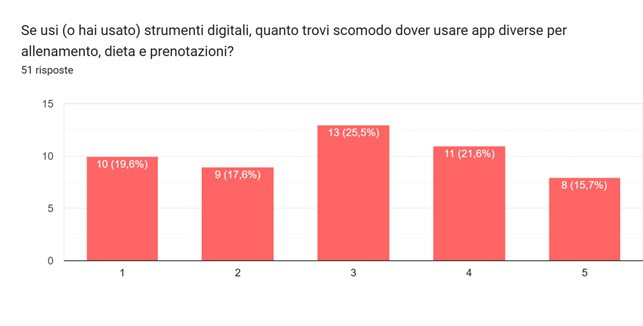
\includegraphics[width=0.8\textwidth]{3-UserResearch/img/Questionnaire/GymMembers/ScomoditaDiverseApp.jpg}
    \caption{Discomforts experienced by gym members when using different fitness apps.}
    \label{img:QuestionnaireDiscomfort}
\end{figure}

\begin{figure}[H]
    \centering
    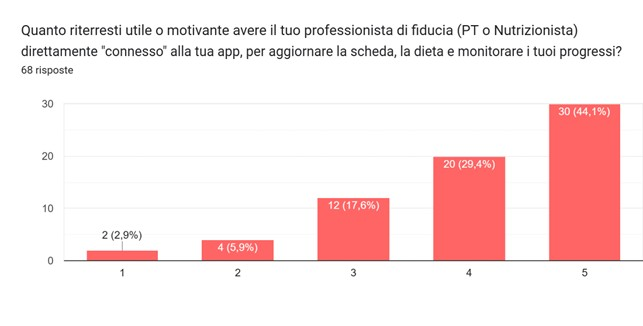
\includegraphics[width=0.8\textwidth]{3-UserResearch/img/Questionnaire/GymMembers/ConnnessioneProfessionista.jpg}
    \caption{Importance of connecting with a fitness professional.}
    \label{img:QuestionnaireConnection}
\end{figure}

\vspace{0.3cm}
\textbf{Analysis of Gym Members' Feedback:} 
The data reveals a highly active user base, with most participants training 2 to 5 times a week (Figure \ref{img:QuestionnaireFrequency}). Despite this dedication, Figure \ref{img:QuestionnaireTracking} highlights a critical inefficiency: a substantial portion of users still relies on analog methods (such as pen and paper or basic phone notes) or completely lacks a structured tracking system. Furthermore, many respondents suffer from the fragmentation of using multiple applications simultaneously. Consequently, Figure \ref{img:QuestionnaireDiscomfort} demonstrates the high frustration caused by this lack of integration. Most importantly, as depicted in Figure \ref{img:QuestionnaireConnection}, users expressed an overwhelming desire to have a direct, digital connection with their trusted professionals to receive updated diets and workout plans without constantly switching platforms.

\paragraph{Open Text Paragraph} Furthermore, the questionnaire included an open-ended question specifically directed at gym members, asking: \textit{"If you use one or more applications, please write their names in the field below"}. This specific inquiry proved to be extremely valuable for our overall market research. It allowed us to deepen and empirically validate the theoretical findings discussed during the Competitor Analysis phase (Chapter \ref{sect:CompetitorsAnalysis}). By collecting the exact names of the tools currently adopted by our real target audience, we were able to cross-reference our initial data, confirm our list of direct and indirect competitors, and ultimately prove the strong fragmentation that characterizes the current digital fitness landscape.


\subsubsection{Professionals' Feedback}\label{subsubsect:Professionals'Feedback}

\begin{figure}[H]
    \centering
    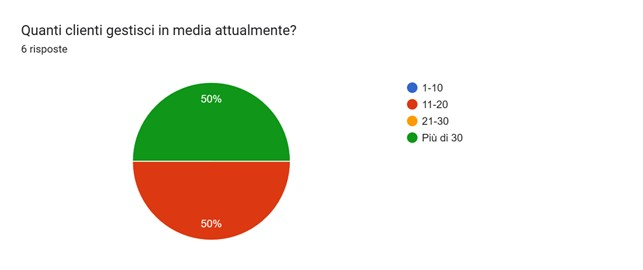
\includegraphics[width=0.8\textwidth]{3-UserResearch/img/Questionnaire/Professionists/NumeroClienti.jpg}
    \caption{Number of clients.}
    \label{img:QuestionnaireClients}
\end{figure}

\begin{figure}[H]
    \centering
    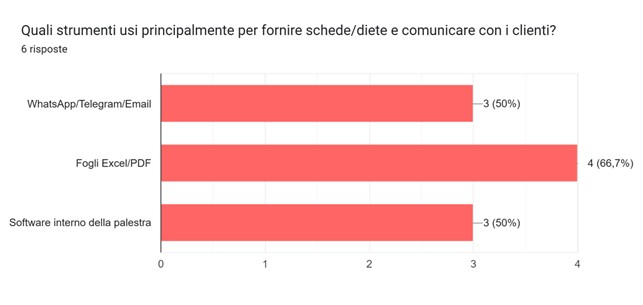
\includegraphics[width=0.8\textwidth]{3-UserResearch/img/Questionnaire/Professionists/StrumentiMonitoraggio.jpg}
    \caption{Tools used for monitoring clients.}
    \label{img:QuestionnaireMonitoring}
\end{figure}

\begin{figure}[H]
    \centering
    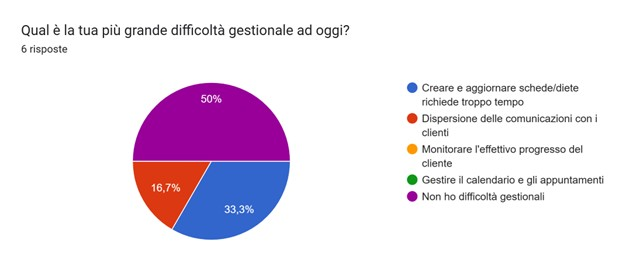
\includegraphics[width=0.8\textwidth]{3-UserResearch/img/Questionnaire/Professionists/DifficoltaGestionale.jpg}
    \caption{Challenges in client management.}
    \label{img:QuestionnaireChallenges}
\end{figure}

\vspace{0.3cm}
\textbf{Analysis of Professionals' Feedback:} 
The surveyed professionals manage varying client loads, ranging from a few individuals up to groups of over 50 clients (Figure \ref{img:QuestionnaireClients}). The core issue disrupting their workflow is clearly identified in Figure \ref{img:QuestionnaireMonitoring}: a heavy reliance on generic, non-specialized tools such as WhatsApp, Telegram, Emails, and Excel spreadsheets. Unsurprisingly, Figure \ref{img:QuestionnaireChallenges} confirms that their primary management challenges revolve around the dispersion of communications and the lack of constant, organized feedback from clients. Managing multiple user routines through chaotic messaging applications creates an unsustainable administrative burden, strongly proving the necessity for a centralized professional dashboard.


\subsubsection{User Expectations and Proposed Solutions}\label{subsubsect:CommonFeedback}

\begin{figure}[H]
    \centering
    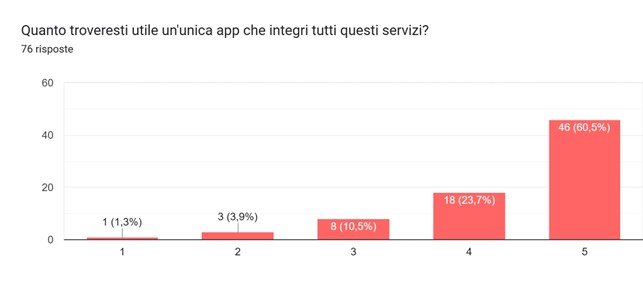
\includegraphics[width=0.8\textwidth]{3-UserResearch/img/Questionnaire/Common/UtilitaIntegrazione.jpg}
    \caption{Perceived usefulness of integrating a fitness app with a professional's monitoring system.}
    \label{img:QuestionnaireIntegration}
\end{figure}

\begin{figure}[H]
    \centering
    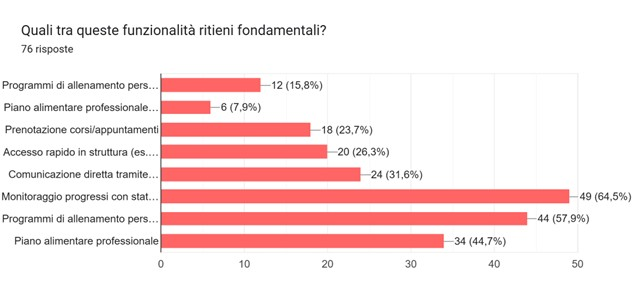
\includegraphics[width=0.8\textwidth]{3-UserResearch/img/Questionnaire/Common/FunzionalitaFondamentali.jpg}
    \caption{Essential features for a fitness app integrated with a professional's monitoring system.}
    \label{img:QuestionnaireEssentialFeatures}
\end{figure}

\vspace{0.3cm}
\textbf{Analysis of Expectations:} 
When asked about the potential utility of an all-in-one application that aggregates all these scattered services, the response was incredibly positive: Figure \ref{img:QuestionnaireIntegration} shows an overwhelming approval rating from both clients and professionals. Regarding the core functionalities (Figure \ref{img:QuestionnaireEssentialFeatures}), respondents pinpointed personalized workout tracking, professional diet management, and rapid digital facility access as absolute must-haves. These results definitively validate our initial feature assumptions and provide a clear, user-approved roadmap for TrainHub's core architecture.

\subsubsection{Qualitative Insights and Methodological Refinement}\label{subsubsect:QualitativeInsights}

\paragraph{Uncovering Unmet Needs and Feature Elicitation}
To maximize the value of our user research, the survey included an open-ended question designed to uncover specific pain points: \textit{"If you could improve or solve an impractical aspect related to the digital experience in the gym, what would it be?"}. Rather than directly asking participants what features they wanted, this problem-oriented approach allowed us to indirectly elicit new and unanticipated functional requirements. By focusing on the users' real frustrations and daily friction points, we gathered organic insights into unmet needs. This qualitative data significantly enriched the conceptualization of TrainHub, helping us identify and prioritize secondary features that could further elevate the platform's value proposition.

\paragraph{Methodological Feedback and Iterative Improvement}
Finally, acknowledging our ongoing learning process as university students, we added a concluding section dedicated entirely to methodological feedback: \textit{"Being a university project, we are still learning how to conduct user research. If you found any question unclear or hard to interpret, please let us know. Every feedback is gold to us!"}. This meta-research inquiry proved to be incredibly valuable in practice. The constructive criticism received from the earliest respondents highlighted minor ambiguities in our initial phrasing. Consequently, we adopted an agile and iterative approach, actively fine-tuning and adjusting the questionnaire during the data collection phase. This continuous refinement ensured maximum clarity for subsequent participants, thereby increasing the overall reliability and accuracy of our final dataset.
\subsection{Affinity Diagram}\label{subsect:AffinityDiagram}
Following the collection of raw data from the survey, we applied the Affinity Diagram methodology to systematically organize facts, opinions, and insights. This collaborative UX mapping activity was executed through a structured 8-step process to synthesize the research findings before defining the User Personas.

\paragraph{Steps 1 \& 2: Data Collection and Sticky Notes Generation}
We began by extracting the most relevant qualitative and quantitative information from the 81 valid questionnaire responses. We translated these data points into virtual sticky notes using \textbf{Figma}. The notes included direct quotes, statistics, and recurring pain points. For instance, client-side notes highlighted phrases like \textit{"I use paper, pen, or phone notes to track my workouts"} or \textit{"Switching between multiple apps for workouts and diets is highly frustrating,"} while professional-side notes emphasized \textit{"WhatsApp and Excel are chaotic for managing multiple clients."}

\paragraph{Steps 3, 4 \& 5: Clustering, Labeling, and Combining}
Once the digital board was populated, we grouped the notes into clusters based on natural relationships and labeled them according to their core themes. By combining similar concepts, three overarching macro-themes emerged:
\begin{itemize}
    \item \textbf{The Burden of Digital Fragmentation:} a massive cluster formed around the inefficiency of current tracking methods. Sticky notes indicating the use of pen and paper, phone notes, and the simultaneous use of multiple apps were combined under this theme. The high frustration scores recorded in the survey strongly validated this label;
    \item \textbf{Inefficient B2C Communication:} this cluster grouped the professionals' administrative struggles (e.g., relying on generic messaging apps) with the clients' desire for a stronger, digital connection with their Personal Trainers. It highlighted the friction in exchanging feedback and updating diet/workout plans;
    \item \textbf{The "All-in-One" Demand:} a solution-oriented cluster aggregating the highly requested core features: unified workout tracking, integrated diet management, and digital facility access via QR code. 
\end{itemize}

\begin{figure}[H]
    \centering
    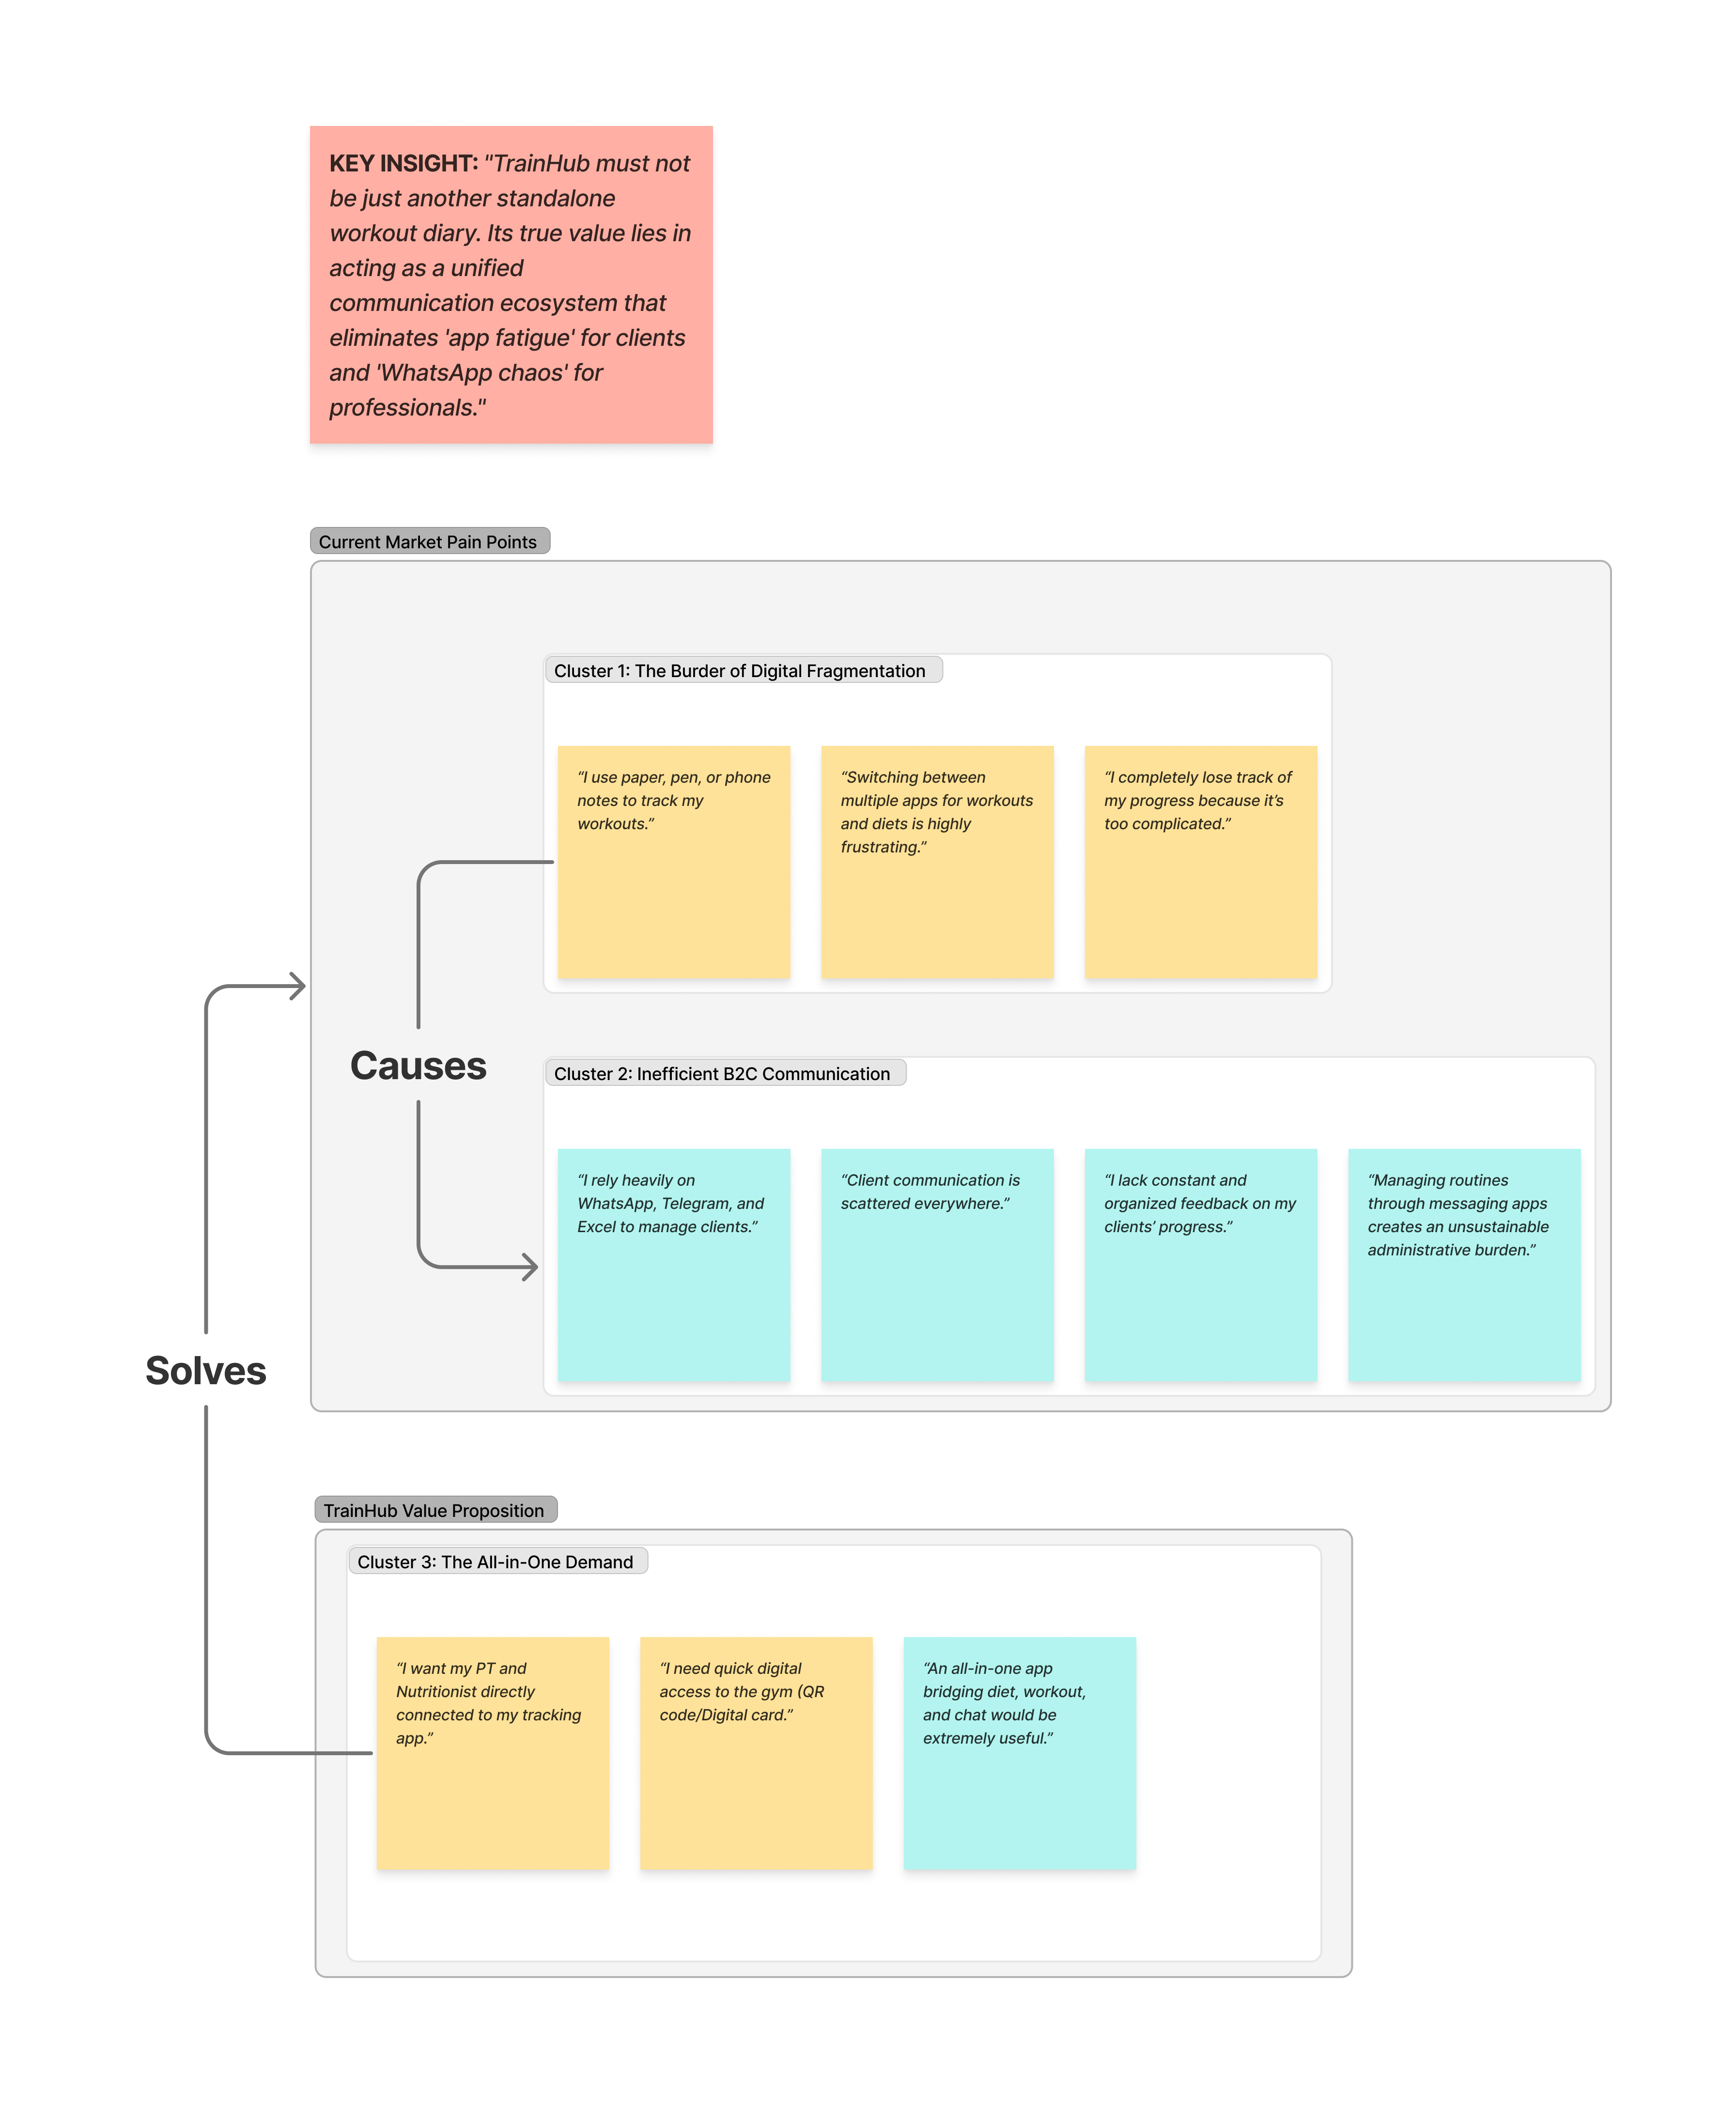
\includegraphics[width=0.9\textwidth]{3-UserResearch/img/AffinityDiagram/AffinityDiagram.jpg}
    \caption{Affinity Diagram board developed in Figma containing the clustered sticky notes.}
    \label{img:AffinityDiagramBoard}
\end{figure}

\paragraph{Step 6: Linking Dependencies}
After defining the macro-themes, we mapped the dependencies between the clusters. The structural link became evident: the \textit{Burden of Digital Fragmentation} (cause) directly forces professionals to resort to \textit{Inefficient B2C Communication} (effect), leading to poor tracking and frustrated users. The \textit{"All-in-One" Demand} acts as the structural bridge capable of resolving these dependencies by unifying the ecosystem.

\paragraph{Steps 7 \& 8: Interpretation and Documentation}
The final interpretation of this affinity mapping exercise provided a clear design directive. The diagram confirmed that TrainHub's core value does not simply lie in offering a digital workout diary, but rather in acting as a centralized communication hub that eliminates the "app fatigue". Documenting this process allowed us to confidently transition from raw, scattered survey data to well-defined, evidence-based user profiles. The insights finalized in this section directly shaped the goals and frustrations of the User Personas presented in the following paragraphs.

\subsection{User Personas}\label{subsect:Personas}

\begin{figure}[H]
    \centering
    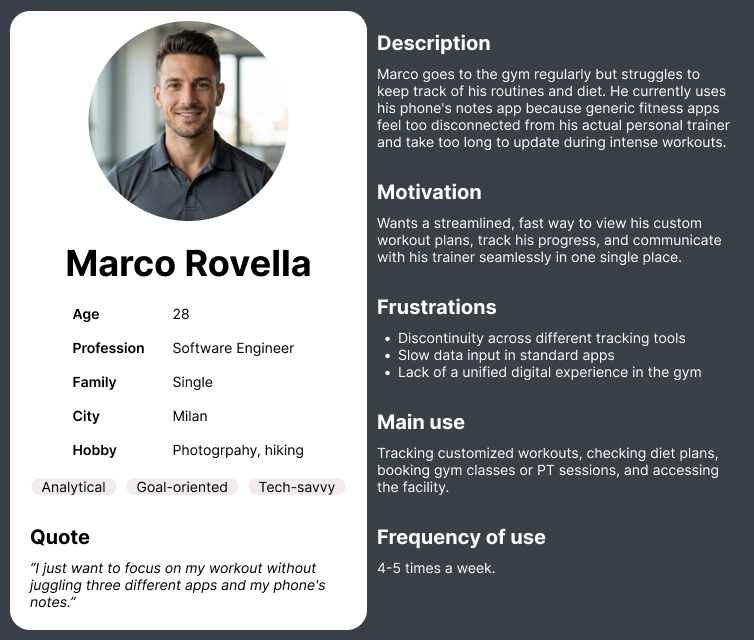
\includegraphics[width=0.8\textwidth]{3-UserResearch/img/Personas/Persona1.jpg}
     \caption{Persona 1: Young Gym Member.}
     \label{fig:Persona1}
\end{figure}

\begin{figure}[H]
    \centering
    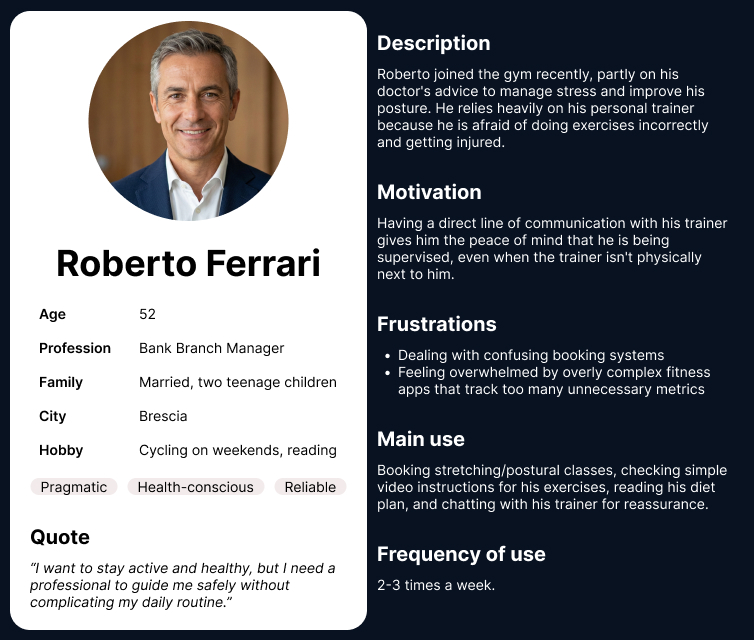
\includegraphics[width=0.8\textwidth]{3-UserResearch/img/Personas/Persona2.jpg}
     \caption{Persona 2: Senior Gym Member.}
     \label{fig:Persona2}
\end{figure}

\begin{figure}[H]
    \centering
    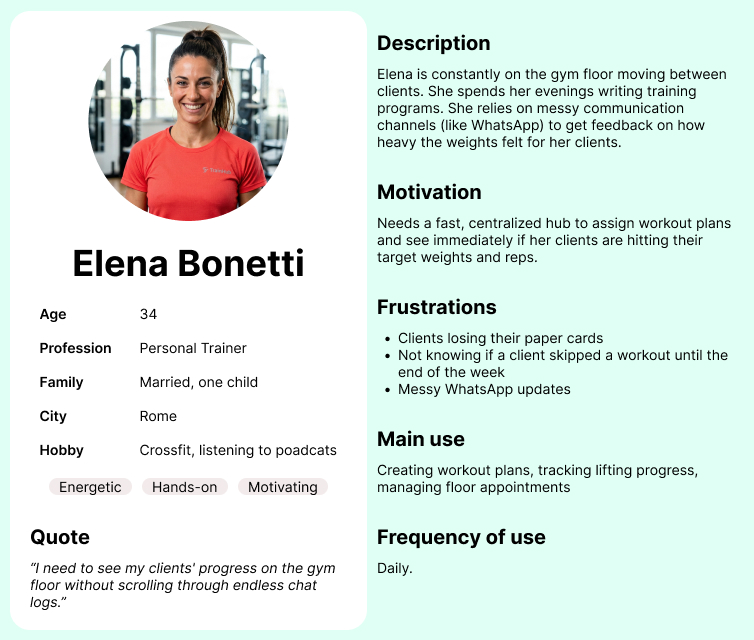
\includegraphics[width=0.8\textwidth]{3-UserResearch/img/Personas/Persona3.jpg}
     \caption{Persona 3: Personal Trainer.}
     \label{fig:Persona3}
\end{figure}

\begin{figure}[H]
    \centering
    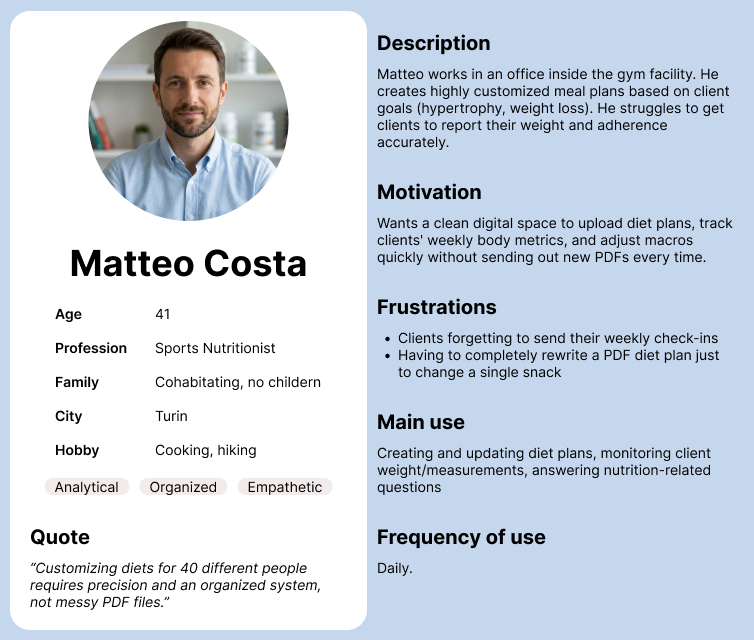
\includegraphics[width=0.8\textwidth]{3-UserResearch/img/Personas/Persona4.jpg}
     \caption{Persona 4: Nutritionist.}
     \label{fig:Persona4}
\end{figure}
\subsection{User Scenarios}\label{subsect:Scenarios}

\paragraph{Scenario 1: Marco Rovella (Young Gym Member)}Marco is in the weight room, in the middle of an intense workout, with limited time before heading back to the office. Marco needs to log the weights for his main exercise (Bench Press) as quickly as possible so he doesn't lose his focus.
Instead of opening his phone's notes app, he unlocks his screen and opens TrainHub, which immediately display today's routine. With a couple of quick taps on the “+” and “-” buttons, he confirms the pre-filled weights assigned by his PT based on his last session, marks the set as complete, and immediately moves on to the next exercise, receiving a small virtual badge for his consistency.

\paragraph{Scenario 2: Roberto Ferrari (Senior Gym Member)}It is Tuesday evening and Roberto is at home, relaxing on the couch after dinner. Roberto wants to prepare for tomorrow's workout and make sure he performs the exercises correctly to avoid hurting his back.
He opens the TrainHub app on his smartphone and he accesses his customized workout plan and watches a short video demonstration of an assigned exercise. Feeling a bit unsure about a specific movement, he uses the app's built-in chat to send a quick message to his PT (Elena), asking if the movement is appropriate for his level, and immediately feels reassured.

\paragraph{Scenario 3: Elena Bonetti (Personal Trainer)}Elena is on the gym floor, enjoying a short 5-minute break between one client and the next. Elena needs to monitor the progress of her clients who are working out independently to see if the assigned weights are appropriate. She pulls her phone out of her pocket and opens the TrainHub Admin dashboard. She sees a notification indicating that Marco has just completed his workout, hitting his target weights. Without having to open messy WhatsApp chats or Excel spreadsheets, Elena taps on Marco's profile and directly modifies the parameters of his routine for the following week, slightly increasing the load. She saves the changes is seconds, ready to welcome her next in-person client.

\paragraph{Scenario 4: Matteo Costa (Nutritionist)}It is Friday morning and Matteo is in his tidy offce inside the fitness facility. Matteo must analyze his clients' weekly weight check-ins and update their diet plans ahead of the weekend.
He logs into the TrainHub web app from his laptop. His main dashboard displays an automated summary showing who has logged their weight and who hasn't. Noticing that Roberto has entered his data but hit a plateau, Matteo accesses his digital nutrition plan and quickly adjusts the carbohydrate macros for his dinners. With a single click, he saves and publishes the new diet without needing to generate or email any PDF files. The system automatically sends a push notification to Roberto.